\documentclass[]{report}
\usepackage[utf8]{inputenc}
\usepackage{graphicx}

\title{Akonadi\\The PIM storage framework for KDE 4}
\author{Tobias Koenig}

\begin{document}

\maketitle

\tableofcontents

\chapter{Introduction}

During the last 5 years, after the release of KDE 3.0, the requirements of our users
have constantly increased. When it was OK that our PIM solution was able to handle 100 contacts,
300 events and maybe 1000 Mails in 2001, nowadays user expect that the software is able to
handle a multiple of it. Over the years the KDE PIM developer tried to catch up with the new
requirements, however since KDE 3.x had to stay binary compatible they were limited in their
efforts.

With the new major release KDE 4.0 it's possible to completely redesign the PIM libraries from
ground up and using new concepts to face the requirements in 2006 and beyond.

\section{General}

After some discussion at the yearly KDE PIM meeting in Osnabrück in January 2006 the PIM developers
came to the conclusion that a service is needed which acts as a local cache on the users desktop
and provides search facilities. The name Akonadi comes from a divinity from Ghana and was chosen since
all other nice names were already used by other projects in the Internet ;)

\section{Problems with implementation of KDE 3.x}

Before digging into the internal of Akonadi we want to take a look at the implementation of the
old KDE PIM libraries to understand the problems and conceptual shortcomings.

The main PIM libraries libkabc (contacts) and libkcal (events) where designed at a time when the
address book and calendar where files on the local file system, so there was no reason to think
about access time and mode. The libraries accessed the files synchronously and loaded all data of the
file into memory to be able to perform search queries on the data set. It worked well for local files
but over time plug-ins for loading data from groupware server were written, so the synchronous access blocked
the application which used libkabc/libkcal and loading all 2000 contacts from a server is not only
time consuming but also needs a lot of memory to store them locally. The KDE PIM developer tried to
address the first issue by adding an asynchronous API, but it was not well implemented and difficult to use.
At the end, the design decision caused the following problems:

\begin{itemize}
  \item Bad Performance
  \item Hugh Memory Consumption
\end{itemize}

Another important but missing thing in the libraries were support for notifications and locking.
The former was partly implemented (at least reflected by the API) but only implemented in the local
file plug-in, so it was practical unusable. The latter was also partly implemented but never really tested and
lead to deadlocks sometimes, so the following problems appeared as well:

\begin{itemize}
  \item Missing Notifications
  \item Missing Locking
\end{itemize}

The main aim of Akonadi is to solve these issues and make use of the goodies of the new design brings.

\chapter{Concepts}

\section{Basic Thoughts}

To solve the problems mentioned above and make Akonadi ready for the requirements of the KDE 4 release
cycle, some considerations had been made which had a deep influence on the design:

\begin{itemize}
  \item \textbf{Functionality is spread into different processes}\\
        This separation has the big advantage that if one process crashes because of
        a programming error it doesn't effect the other components. That results in
        robustness of the whole system. A disadvantage might be that there is an additional
        overhead for inter-process communication.
  \item \textbf{Communication protocol is split into data and control channel}\\
        When doing communication between processes you have to differ between the type of data
        that should be are transferred. For a large amount of data a high-performance
        protocol should be used and for control data a low-latency protocol.
        Matching both requirements in one protocol is mostly impossible and hard to
        achieve with currently available software.
  \item \textbf{Separate logic from storage}\\
        By separating the logic from the storage, the storage can be used to store data
        of any type. In this case, the storage is a kind of service, which is available for
        other components of the system. The logic is located in separated components and so
        3rd-party developer can extend the system by providing their own components.
  \item \textbf{Keep communication asynchronous}\\
        To allow a non-blocking GUI all the communication with the back-end and within the
        back-end itself must be asynchronous. For the application developer you can easily
        provide a synchronous convenience API, however the back-end must communicate asynchronously.
\end{itemize}

Keep these considerations in mind when you read the following design concept.

\section{Schema}

In the diagram below you can see a rough concept of structure of Akonadi:

\begin{center}
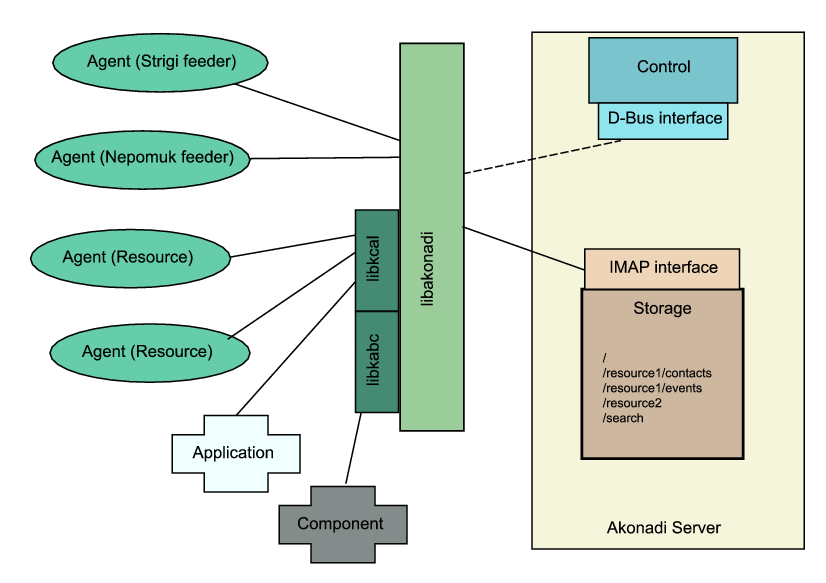
\includegraphics[height=6cm]{pics/concept.png}
\end{center}

The main components are:
\begin{itemize}
  \item Storage
  \item Control
  \item Agents (Resources)
  \item SearchProviders
  \item libakonadi
\end{itemize}

\subsection{The Storage}
The Storage is a process which provides an API for store arbitrary data over
an IMAP interface. The advantage of IMAP is the mature state of the protocol
and its capability to handle a huge amount of data.
Whenever new items are added to the Storage or removed from, the Storage will
emit a signal over its DBus-Interface to inform other components.
As defined in the IMAP standard, also a simple type of search is supported,
so you can query for all items of a special mime-type or email specific fields.
For more complex search queries, another component, the SearchProvider, is included.

\subsection{Agents}
Agents are processes which are controlled by the Akonadi server itself and which
are able to work on the cache of the Storage. In the current design there are two
types of Agents:

\begin{itemize}
  \item Autonomous Agents
  \item Resources
\end{itemize}

Autonomous Agents are processes which only work on the cache of the Storage
and the user will seldom or never see them during work.

Resources are processes which load data from an external data source, store them
in the cache of the Storage and keep track of changes on both sides to keep
the external data source and the cache synchronized.
Resources can be grouped to profiles where one Resource can be part of different
profiles. Profiles are useful in use cases like this:
You have configured a local Resource and a groupware server Resource. You want both
to be shown in the address book application but for synchronization with your mobile
phone only the data from the local Resource are from interest. So the easy solution
is to create a profile 'VIEW' where both the local Resource and the groupware server
Resource are part of and a profile 'SYNCHRONIZE' where only the local Resource is
assigned. Now you just have to tell the application which profile it shall use to
access the data.

\subsection{The Control}
The Control process is the 'brain' of the system. It starts the Storage and Resource
processes and monitors them, so if one of these processes crashes, it restarts them immediately.
Furthermore it provides a DBus-API with the following functionality:

\begin{itemize}
  \item Managing Resources
  \item Managing Profiles
  \item Notifications when the state of Resources or Profiles have changed
\end{itemize}

The Control should be started in the startkde script and terminated at the end of the session.

\subsection{The SearchProviders}
As mentioned before the Storage provides only a basic support for search queries. It's limited
to mime types and email specific fields. However to query for contacts or events which match
a specific criterion a more advanced query language is needed. Since this language will contain
domain specific information (like telephon number or start date) but the Storage has no knowledge
about the data it stores, so it can't handle the queries itself.
For more robustness the handling of these queries is put into a separated process and these processes
are called SearchProviders.

\subsection{libakonadi}
Every client application can access the Akonadi service directly via DBus and IMAP API, however
for easier implementation and a better abstraction the library libakonadi is provided which does
all the low level stuff and provides a Qt based API for all the functionality Akonadi provides.
libakonadi works on any type of data and knows nothing about the domain the data are part of.
For the domain specific tasks libkabc and likcal should be used, which are located above the
libakonadi and do the data conversion from the storage format to a Qt/KDE one.

\chapter{Implementation}

\section{Source Code Layout}
All the source code of Akonadi is currently located in KDE SVN repository under
trunk/KDE/kdepim/akonadi and has the following code layout:

\begin{itemize}
  \item \textbf{clients}\\
    Contains some client application which make use of libakonadi.
  \begin{itemize}
    \item \textbf{akonadi}\\
      Contains a command line tool which allows you to communicate with the
      storage to store and retrieve data.
    \item \textbf{akonadiconsole}\\
      Contains a debugging tool for managing Resources and Profiles.
    \item \textbf{kagenda}\\
      Contains an example application of how the calendar interface in KDE 4
      could look like.
  \end{itemize}
  \item \textbf{doc}\\
    Contains the \LaTeX sources of this document.
  \item \textbf{libakonadi}\\
    Contains the library which does the low level communication with the
    Akonadi service.
  \begin{itemize}
    \item \textbf{components}\\
      Contains easy to use widget components which fulfill special tasks like
      selecting a contact or editing an event.
  \end{itemize}
  \item \textbf{resources}\\
  \begin{itemize}
    \item \textbf{include}\\
      Contains the DBus interface description and header files for the Resource
      base class.
    \item \textbf{src}\\
    \begin{itemize}
      \item \textbf{ical}\\
        Contains the Resource for local iCalendar file.
      \item \textbf{knut}\\
        Contains a debugging and testing Resource.
      \item \textbf{lib}\\
        Contains the implementation of the Resource base class.
    \end{itemize}
  \end{itemize}
  \item \textbf{server}\\
    Contains the source code of the Storage and Control components.
  \begin{itemize}
    \item \textbf{control}\\
      Contains the source code of the Control component.
    \item \textbf{debugger}\\
      Contains the akonadi\_debugger application, a debugger to monitor all the communication
      between Akonadi and its clients.
    \item \textbf{interfaces}\\
      Contains the DBus interface descriptions of the Akonadi components.
    \item \textbf{src}\\
      Contains the source code of the Storage component.
    \begin{itemize}
      \item \textbf{handler}\\
        Contains the source code for the handlers of the single IMAP commands.
      \item \textbf{storage}\\
        Contains the source code for accessing the storage back-end.
    \end{itemize}
  \end{itemize}
\end{itemize}

\chapter{Usage}

\section{How to get started}
To start the Akonadi server you call 'akonadi\_control', which is the Control process,
on the command line, now the Akonadi server is ready be accessed by client applications.

\section{Debugging tools}
From time to time it's necessary to debug the Akonadi system. For this purpose 2 utils are
available:
\begin{itemize}
  \item akonadi\_debugger
  \item akonadiconsole
\end{itemize}

akonadi\_debugger is a tool which shows you the whole communication between the Storage and
the client.
The akonadiconsole is a management tool to create, remove, configure and start synchronization
of Resources. Furthermore you can create and remove profiles with it.

\end{document}
